\documentclass[a4paper,12pt]{article} % добавить leqno в [] для нумерации слева
\usepackage[a4paper,top=1.3cm,bottom=2cm,left=1.5cm,right=1.5cm,marginparwidth=0.75cm]{geometry}
%%% Работа с русским языком
\usepackage{cmap}					% поиск в PDF
\usepackage{mathtext} 				% русские буквы в фомулах
\usepackage[T2A]{fontenc}			% кодировка
\usepackage[utf8]{inputenc}			% кодировка исходного текста
\usepackage[english,russian]{babel}	% локализация и переносы

\usepackage{graphicx}

\usepackage{wrapfig}
\usepackage{tabularx}

\usepackage{hyperref}
\usepackage[rgb]{xcolor}
\hypersetup{
colorlinks=true,urlcolor=blue
}
\usepackage{multirow}
\usepackage{hhline}


%%% Дополнительная работа с математикой
\usepackage{amsmath,amsfonts,amssymb,amsthm,mathtools} % AMS
\usepackage{icomma} % "Умная" запятая: $0,2$ --- число, $0, 2$ --- перечисление

%% Номера формул
\mathtoolsset{showonlyrefs=true} % Показывать номера только у тех формул, на которые есть \eqref{} в тексте.

%% Шрифты
\usepackage{euscript}	 % Шрифт Евклид
\usepackage{mathrsfs} % Красивый матшрифт

%% Свои команды
\DeclareMathOperator{\sgn}{\mathop{sgn}}

%% Перенос знаков в формулах (по Львовскому)
\newcommand*{\hm}[1]{#1\nobreak\discretionary{}
{\hbox{$\mathsurround=0pt #1$}}{}}

\begin{document}
	
	\begin{titlepage}
	\begin{center}
		{\large МОСКОВСКИЙ ФИЗИКО-ТЕХНИЧЕСКИЙ ИНСТИТУТ (НАЦИОНАЛЬНЫЙ ИССЛЕДОВАТЕЛЬСКИЙ УНИВЕРСИТЕТ)}
	\end{center}
	\begin{center}
		{\large Физтех-школа электроники, фотоники и молекулярной физики}
	\end{center}
	
	
	\vspace{4.5cm}
	{\huge
		\begin{center}
			{Лабораторная работа 2.4.1}\\
			Определение теплоты испарения жидкости
		\end{center}
	}
	\vspace{2cm}
	\begin{flushright}
		{\LARGE Салтыкова Дарья \\
			\vspace{0.5cm}
			Б04-105}
	\end{flushright}
	\vspace{8cm}
	\begin{center}
		Долгопрудный 2022
	\end{center}
\end{titlepage}

\section{Введение}

\textbf{Цель работы:} 1) измерение давления насыщенного пара жидкости при разной температуре; 2) вычисление по полученным данным теплоты испарения с помощью уравнения Клапейрона–Клаузиуса.
\medskip

\noindent \textbf{Оборудование:} термостат; герметический сосуд, заполненный исследуемой жидкостью; отсчетный микроскоп.
\medskip

\section{Теоретические сведения}

Теплоту парообразования жидкостей можно измерить непосредственно при помощи калориметра. Такой метод, однако, не позволяет получить точных результатов из-за неконтролируемых потерь тепла, которые трудно сделать малыми. В настоящей работе для определения теплоты испарения применен
косвенный метод, основанный на формуле Клапейрона–Клаузиуса: $$\frac{dP}
{dT} = \frac{L}{T(V_2 - V_1)}\;(1).$$
Здесь $P$ — давление насыщенного пара жидкости при температуре $T$, $T$ — абсолютная температура жидкости и пара, $L$ — теплота испарения жидкости, $V2$ — объем пара, $V1$ — объем жидкости. Найдя из опыта $\frac{dP}{dT},\; T,\; V2$ и $V1$, можно определить $L$ путем расчета. Величины $L, \;V2$ и $V1$ в формуле (1) должны относиться к одному и тому же количеству вещества; мы будем относить их к одному молю.
В нашем приборе измерения производятся при давлениях ниже атмосферного. В этом случае задача существенно упрощается.

С помощью уравнения Ван-дер-Ваальса можно получить зависимость P(T), с помощью которой определить искомую величину:

$$(P+\frac{a}{V^2})(V-b)=RT \; (2)$$
В таблице ниже приведены все значения параметров различных жидкостей уранения Ван-дер-Ваальса в условиях данного опыта.
\begin{figure}[h]
	\center{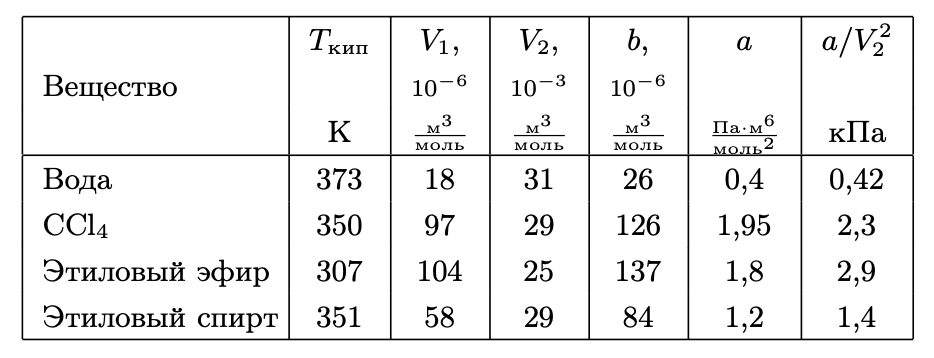
\includegraphics[scale=1]{таблица}}
\end{figure}

Откуда видно, что $\frac{V_1}{V_2} < 0.005$, a $\frac{a}{PV^2}<0.03$, ошибка метода измерений равна 4\%, тогда записав уравнение Клапейрона-Менделеева для насыщенного пара, получим:
$V=\frac{RT}{P}\;.$
Пренебрегая $V_1$ (который не превосходит $0,5\%$ от $V_2$), запишем:
$$L=\frac{RT^2}{P} \frac{dP}{dT} = -R\frac{d(lnP)}{d(1/T)}\;(3).$$
Эта формула является окончательной.

\medskip

\section{Экспериментальная установка}

Схема установки изображена на рисунке. Наполненный водой резервуар 1 играет роль термостата. Нагревание термостата производится спиралью 2, подогреваемой электрическим током. Для охлаждения воды в термостате через змеевик 3 пропускается водопроводная вода. Вода в термостате перемешивается воздухом,
поступающим через трубку 4. Температура воды измеряетс
я термометром 5. В термостат погружен запаянный прибор 6 с исследуемой жидкостью - водой. Над ней находится насыщенный пар (перед заполнением прибора воздух из него был откачан).
Давление насыщенного пара определяется по ртутному манометру,соединенному с исследуемым объемом. Отсчет показаний манометра производится при помощи микроскопа.

\medskip

\noindent Описываемый прибор обладает важным недостатком: термометр определяет температуру термостата, а не исследуемой жидкости (или ее пара). Эти температуры близки друг к другу, если нагревание происходит достаточно медленно. Убедиться в том, что нагревание не является слишком быстрым, можно, сравнивая результаты, полученные при нагревании и при остывании прибора.

\begin{figure}[h]
	\center{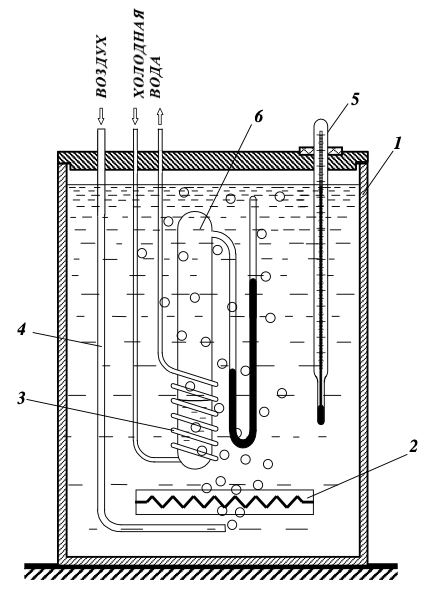
\includegraphics[scale=1]{установка}}
	\caption{Схема установки для определения теплоты испарения}
\end{figure}

\medskip

\section{Ход работы}

1. Измерим разность уровней в ртутном U-образном манометре с помощью микроскопа и температуру по термометру.

\medskip

\noindent 2. Будем нагревать воду в калориметре, пропуская ток через нагреватель. Измерять давление будем с интервалом в 1$^\circ\text{C}$.

\medskip

\begin{tabular}{|c|c|c|c|c|c|c|c|c|c|}
\hline 
$T, ^\circ \text{C}$ & 21,1 & 22 & 23 & 24 & 25 & 26 & 27 & 28 & 29 \\ 
\hline 
$T, K$ & 294,1 & 295 & 296 & 297 & 298 & 299 & 300 & 301 & 302 \\ 
\hline 
$\sigma_T$, K & \multicolumn{9}{c|}{$0,2$} \\ 
\hline 
 & 20,1 & 20,8 & 21,8 & 22,0 & 23,6 & 26,2 & 26,5 & 28,3 & 29,2 \\ 
\hhline{~---------} 
$P', \text{мм}$ & 20,1 & 20,8 & 21,8 & 22,1 & 23,7 & 26,2 & 26,6 & 28,3 & 29,2 \\ 
\hhline{~---------}  
$\text{рт ст}$ & 20,1 & 20,7 & 21,8 & 22,1 & 23,6 & 26,2 & 26,6 & 28,3 & 29,2 \\ 
\hhline{~---------} 
 & 20,0 & 20,8 & 21,8 & 22,1 & 23,6 & 26,2 & 26,6 & 28,3 & 29,2 \\ 
\hhline{~---------} 
 & 20,1 & 20,7 & 21,8 & 22,1 & 23,6 & 26,2 & 26,6 & 28,4 & 29,2 \\ 
\hline 
$\langle P \rangle, \text{Па} $ & 2659 & 2749 & 2887 & 2924 & 3128 & 3470 & 3520 & 2750 & 3867 \\ 
\hline 
$\sigma_P, \text{Па}$ & 26,59 & 26,65 & 26,48 & 26,60 & 26,60 & 26,48 & 26,59 & 26,59 & 26,48 \\ 
\hline 
$ln{P}$ & 7,88 & 7,92 & 7,97 & 9,98 & 8,04 & 8,15 & 8,17 & 8,22 & 8,26 \\ 
\hline 
$\sigma_{ln_P}, *10^{-3}$ & 10,2 & 9,7 & 9,2 & 9,2 & 9,1 & 8,5 & 7,6 & 7,5 & 7,1 \\ 
\hline 
$1/T, 10^{-3}*K^{-1}$ & 3,40 & 3,39 & 3,378 & 3,367 & 3,356 & 3,344 & 3,33 & 3,322 & 3,311 \\ 
\hline 
\end{tabular} 

\medskip
\medskip

\begin{tabular}{|c|c|c|c|c|c|}
\hline 
$T, ^\circ \text{C}$ & 30 & 31 & 32 & 33 & 34 \\ 
\hline 
$T, K$ & 303 & 304 & 305 & 306 & 307 \\ 
\hline 
$\sigma_T$, K & \multicolumn{5}{c|}{0,2} \\ 
\hline 
 & 31,3 & 33,4 & 34,8 & 35,1 & 39,8 \\ 
\hhline{~-----} 
$P', \text{мм}$ & 31,3 & 33,4 & 34,8 & 35,1 & 39,8	 \\ 
\hhline{~-----}  
$\text{рт ст}$ & 31,2 & 33,4 & 34,8 & 35 & 39,8 \\ 
\hhline{~-----} 
 & 31,3 & 33,4 & 34,9 & 35,1 & 39,8 \\ 
\hhline{~-----} 
 & 31,3 & 33,4 & 34,9 & 35,1 & 39,8 \\ 
\hline 
$\langle P \rangle, \text{Па} $ & 4142 & 4423 & 4611 & 4640 & 5270 \\ 
\hline 
$\sigma_P, \text{Па}$ & 26,59 & 26,64 & 26,59 & 26,64 & 26,48 \\ 
\hline 
$ln{P}$ & 8,32 & 8,39 & 8,43 & 8,44 & 8,57 \\ 
\hline 
$\sigma_{ln_P}, *10^{-3}$ & 6,8 & 6,4 & 5,9 & 5,7 & 5,1 \\ 
\hline 
$1/T, 10^{-3}*K^{-1}$ & 3,30 & 3,289 & 3,279 & 3,268 & 3,257 \\ 
\hline 
\end{tabular}

\medskip
\medskip

\noindent 3. Проведем те же измерения при охлаждении жидкости.

\medskip

\begin{tabular}{|c|c|c|c|c|c|c|c|c|c|}
\hline 
$T, ^\circ \text{C}$ & 21 & 22 & 23 & 24 & 25 & 26 & 27 & 28 & 29 \\ 
\hline 
$T, K$ & 294 & 295 & 296 & 297 & 298 & 299 & 300 & 301 & 302 \\ 
\hline 
$\sigma_T$, K & \multicolumn{9}{c|}{$0,2$} \\ 
\hline 
 & 20,5 & 21,2 & 22,5 & 23,3 & 25,2 & 26,4 & 27,3 & 28,4 & 30,3 \\ 
\hhline{~---------} 
$P', \text{мм}$ & 20,4 & 21,2 & 22,6 & 23,3 & 25,2 & 26,3 & 27,3 & 28,5 & 30,3 \\ 
\hhline{~---------}  
$\text{рт ст}$ & 20,4 & 21,2 & 22,5 & 23,3 & 25,3 & 26,4 & 27,3 & 28,5 & 30,2 \\ 
\hhline{~---------} 
 & 20,4 & 21,2 & 22,5 & 23,3 & 25,2 & 26,5 & 27,3 & 28,4 & 30,3 \\ 
\hhline{~---------} 
 & 20,5 & 21,2 & 22,5 & 23,3 & 25,2 & 26,4 & 27,3 & 28,4 & 30,2 \\ 
\hline 
$\langle P \rangle, \text{Па} $ & 2706 & 2807 & 2982 & 3085 & 3340 & 3496 & 3615 & 3766 & 4007 \\ 
\hline 
$\sigma_P, \text{Па}$ & 26,65 & 26,48 & 26,59 & 26,48 & 26,59 & 26,75 & 26,48 & 26,64 & 26,65 \\ 
\hline 
$ln{P}$ & 7,90 & 7,94 & 8,00 & 8,03 & 8,11 & 8,15 & 8,19 & 8,23 & 8,29 \\ 
\hline 
$\sigma_{ln_P}, *10^{-3}$ & 6,6 & 7,1 & 7,6 & 7,9 & 8,6 & 8,9 & 9,4 & 9,8 & 9,8 \\ 
\hline 
$1/T, 10^{-3}*K^{-1}$ & 3,40 & 3,39 & 3,378 & 3,367 & 3,356 & 3,344 & 3,33 & 3,322 & 3,311 \\ 
\hline 
\end{tabular} 

\medskip
\medskip
\medskip

\begin{tabular}{|c|c|c|c|c|c|}
\hline 
$T, ^\circ \text{C}$ & 30 & 31 & 32 & 33 & 34 \\ 
\hline 
$T, K$ & 303 & 304 & 305 & 306 & 307 \\ 
\hline 
$\sigma_T$, K & \multicolumn{5}{c|}{0,2} \\ 
\hline 
 & 31,9 & 34,9 & 36,2 & 37,4 & 39,8 \\ 
\hhline{~-----} 
$P', \text{мм}$ & 32,0 & 34,9 & 36,2 & 37,4 & 39,8	 \\ 
\hhline{~-----}  
$\text{рт ст}$ & 32,0 & 34,9 & 36,2 & 37,3 & 39,8 \\ 
\hhline{~-----} 
 & 32,0 & 34,9 & 36,3 & 37,4 & 39,8 \\ 
\hhline{~-----} 
 & 32,0 & 34,9 & 36,3 & 37,4 & 39,8 \\ 
\hline 
$\langle P \rangle, \text{Па} $ & 4235 & 4621 & 4799 & 4950 & 5271 \\ 
\hline 
$\sigma_P, \text{Па}$ & 26,59 & 26,48 & 26,64 & 26,59 & 26,49 \\ 
\hline 
$ln{P}$ & 8,57 & 8,51 & 8,48 & 8,44 & 8,35 \\ 
\hline 
$\sigma_{ln_P}, *10^{-3}$ & 5,2 & 5,4 & 5,6 & 5,7 & 6,3 \\ 
\hline 
$1/T, 10^{-3}*K^{-1}$ & 3,30 & 3,289 & 3,279 & 3,268 & 3,257 \\ 
\hline 
\end{tabular}

\medskip
\medskip
\medskip
\medskip

\noindent Погрешность измерения давления оценим по формулам 

\medskip

\begin{equation}
\sigma_{P}^{\text{случ}} = \sqrt{\frac{1}{N(N-1)}\sum\limits_{k=1}^N\left(P_k-\langle P \rangle\right)^2}
\end{equation}

\medskip

\begin{equation}
\sigma_{P}^\text{сист} \approx 0,2 \text{ мм рт ст} = 2,65 \text{ Па}
\end{equation}

\medskip

\begin{equation}
\sigma_{P}=\sqrt{(\sigma_{P}^\text{сист})^2 + (\sigma_{P}^\text{случ})^2}
\end{equation}

\medskip

$$\sigma_{\ln{\frac{P}{P_0}}} = \frac{\sigma_P}{P} $$

\medskip
\medskip


\noindent 4. Построим графики в координатах $T$, $P$ и в координатах $\frac{1}{T}, \; ln P$. На графики нанесём точки, полученные при нагревании и охлаждении жидкости.

\medskip

\begin{minipage}{.50\textwidth}
  \centering
  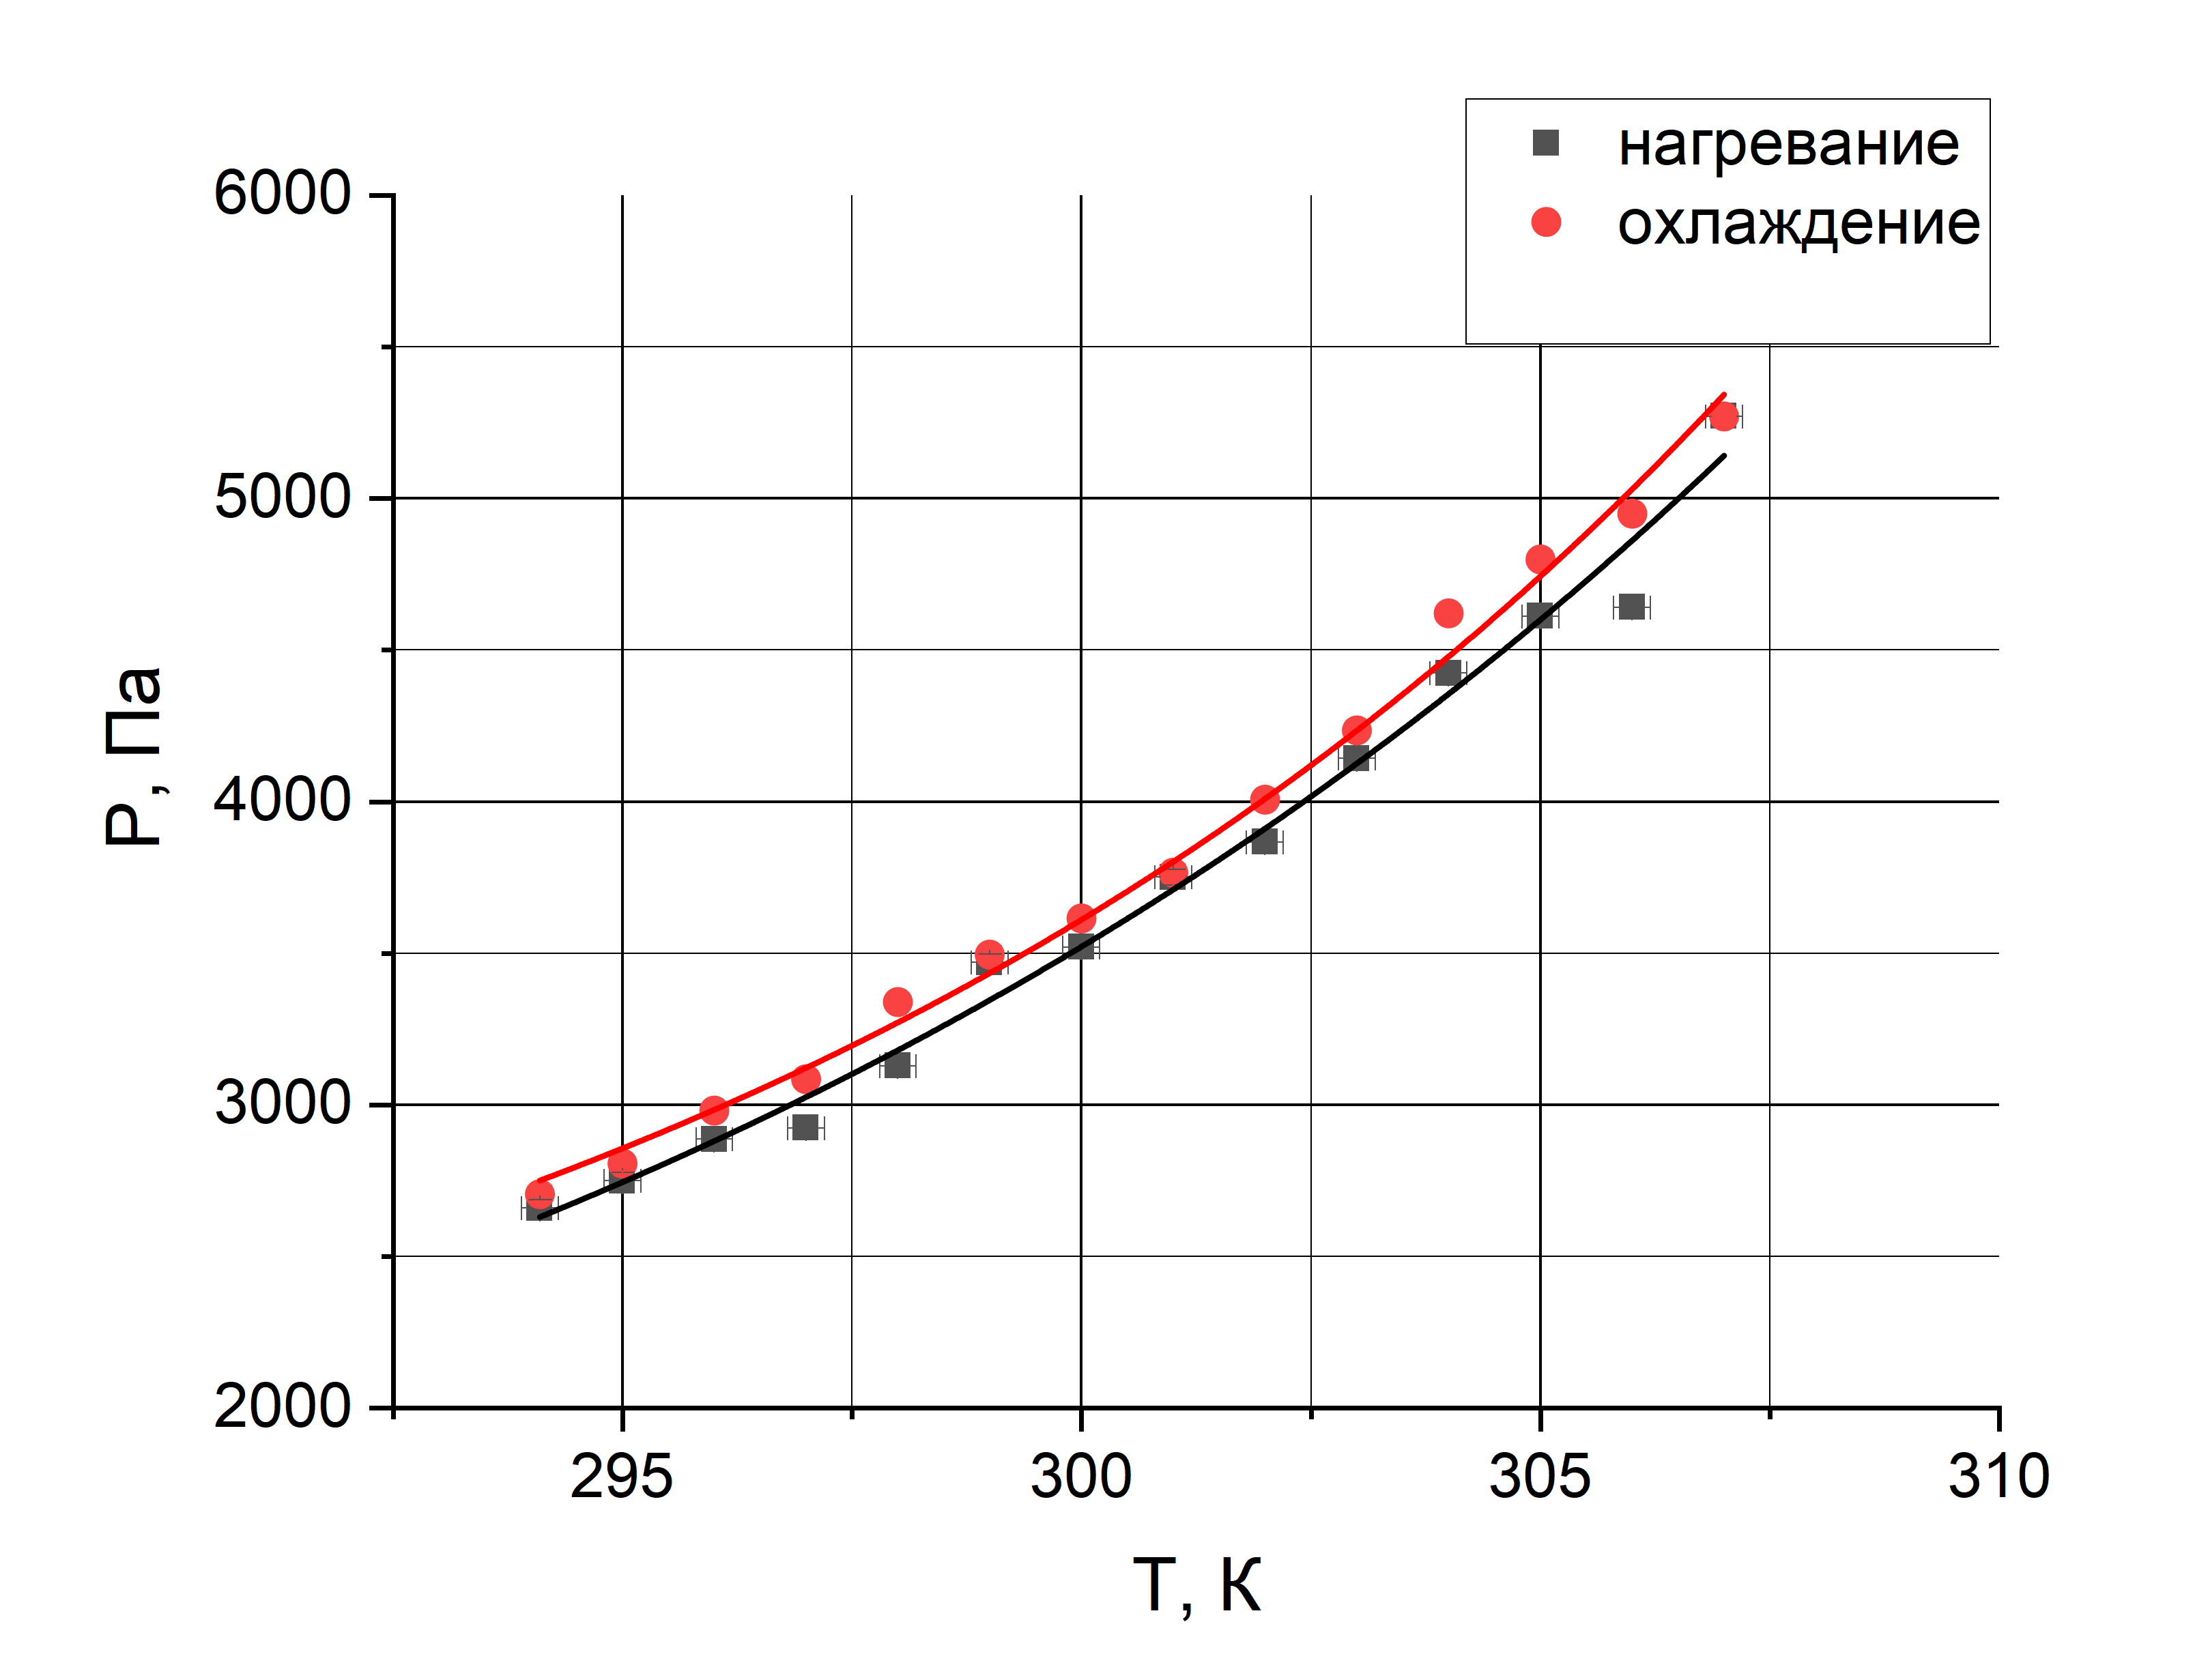
\includegraphics[scale={0.5}]{3.png}
\end{minipage}


\begin{minipage}{.50\textwidth}
  \centering
  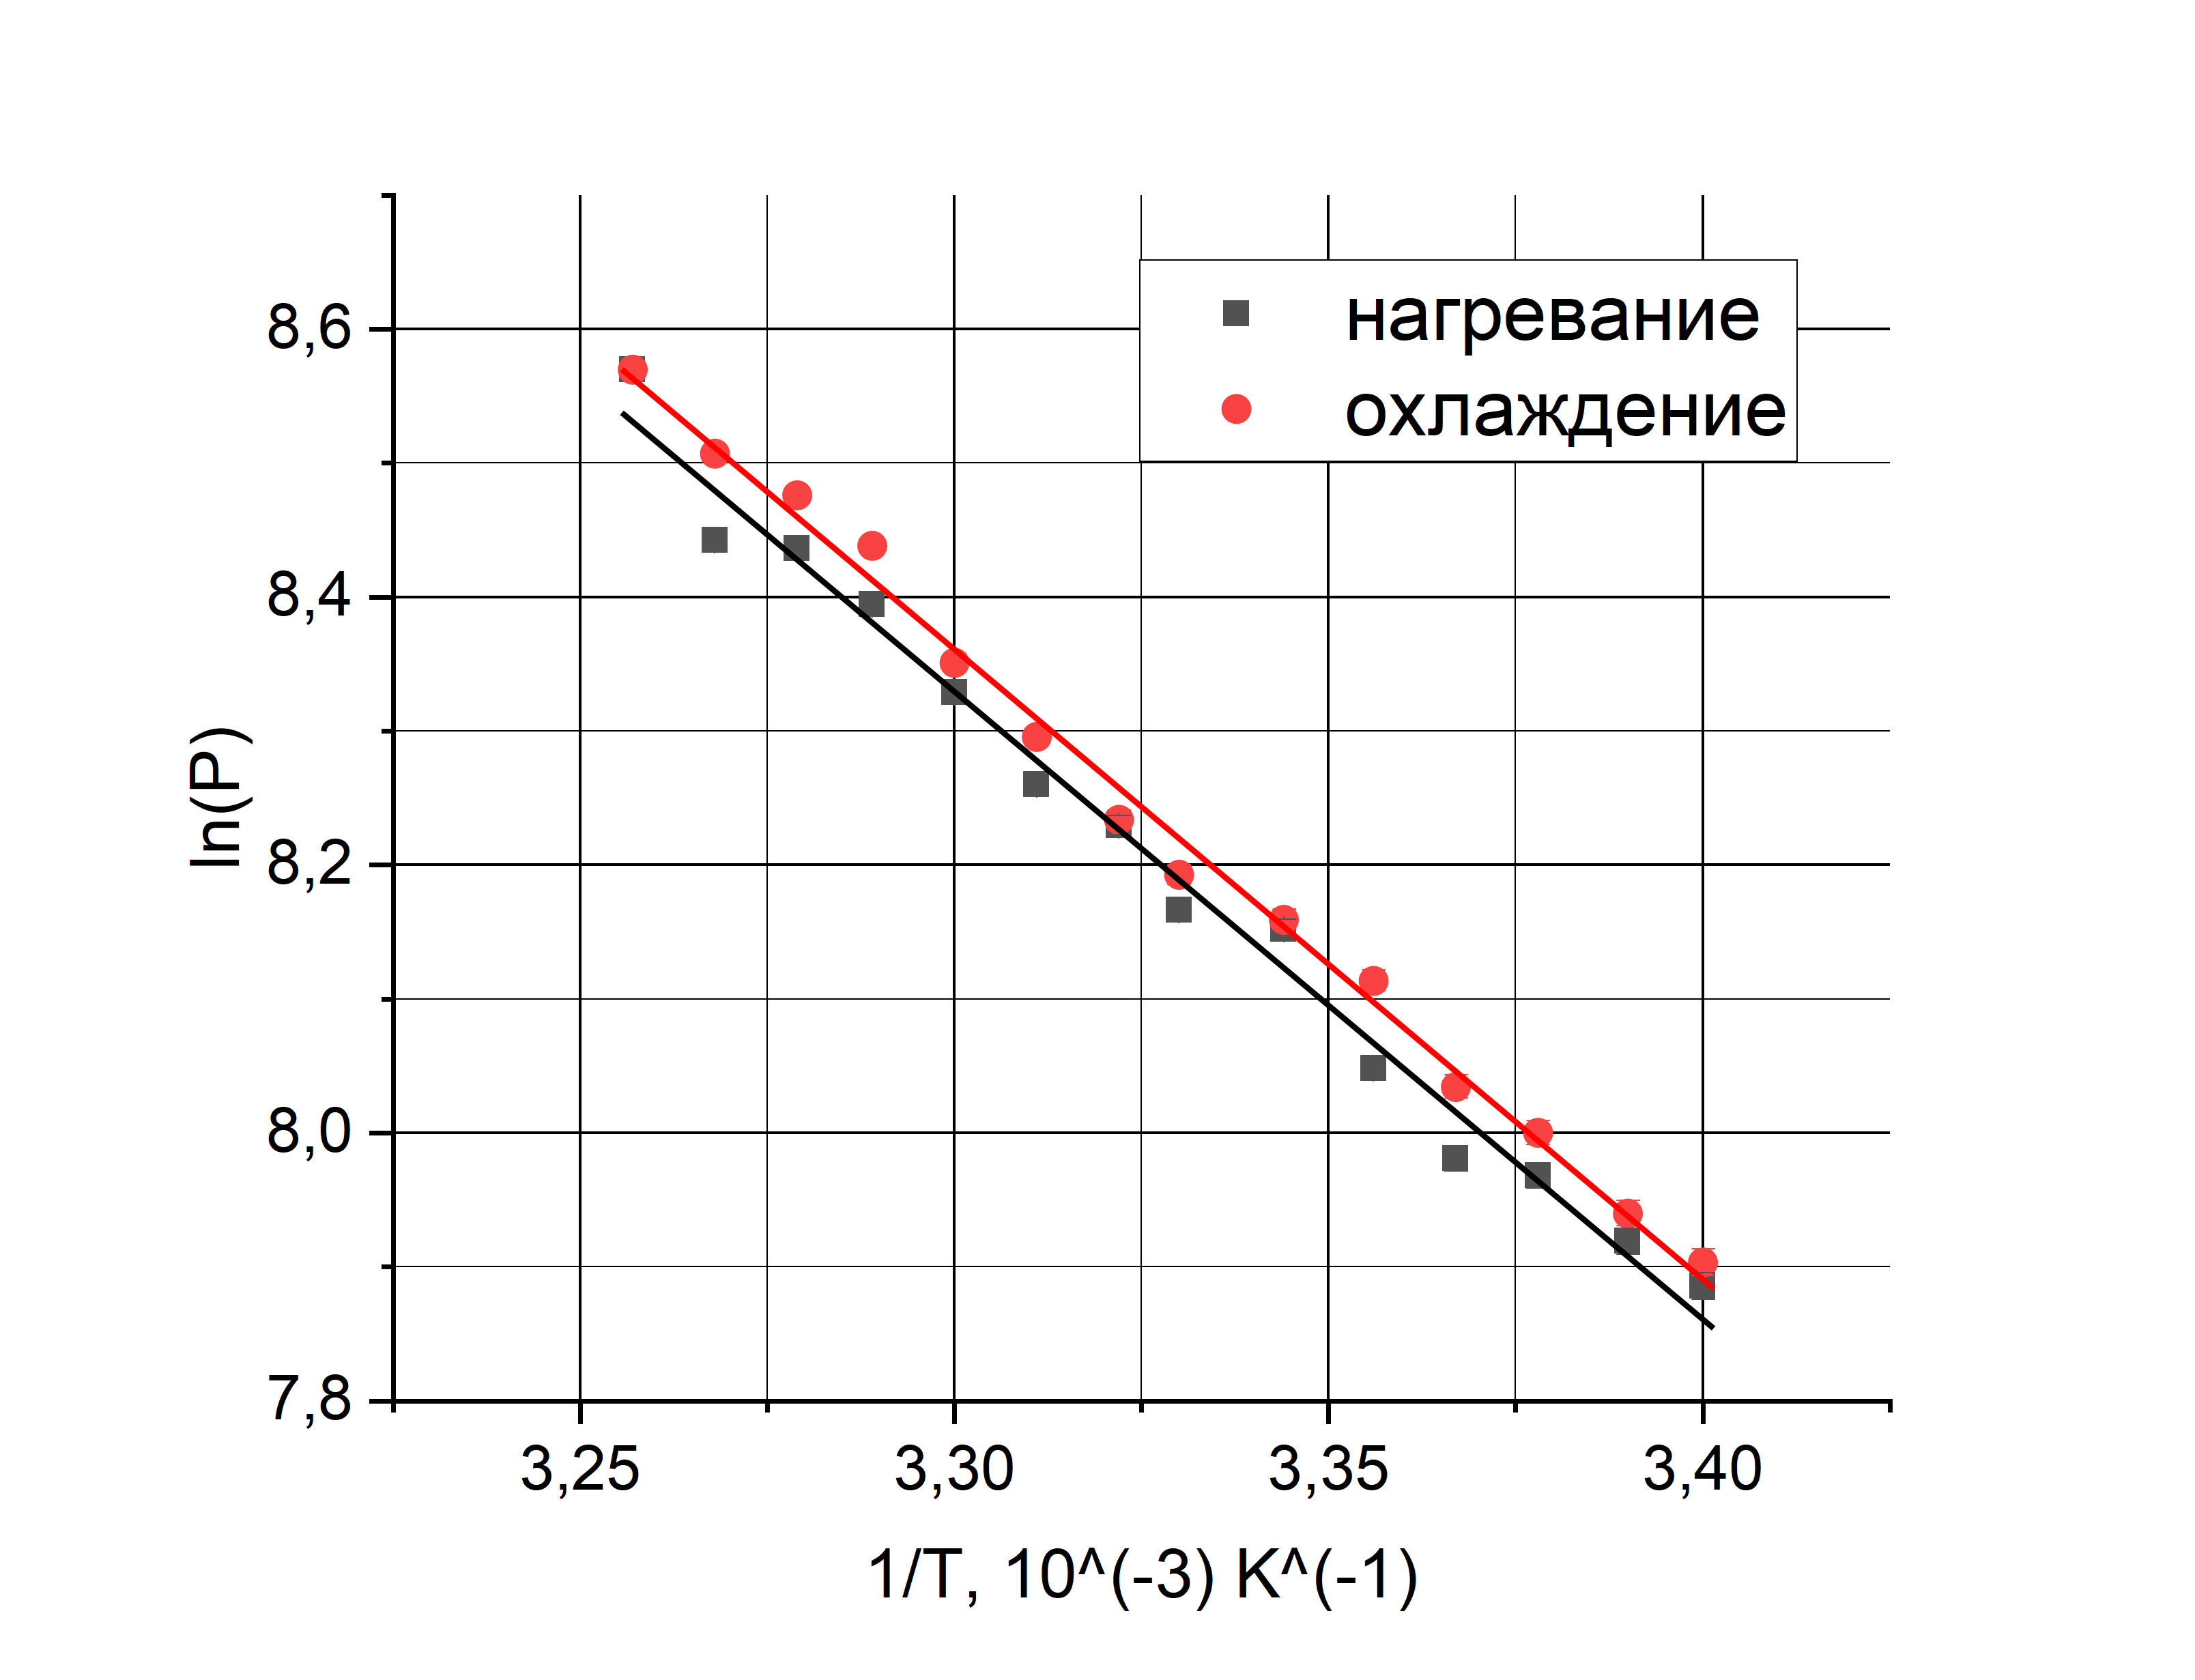
\includegraphics[scale={0.5}]{2.png}
\end{minipage}

\medskip

\noindent По формуле (3) вычислим $L$.
 
\medskip

\noindent Сначала воспользуемся данными первого графика. Аппроксимируем методом наименьших квадратов полученные на этом участке температур зависимости функциями вида \[ P=ae^{bT}, \] где $ a $ и $ b $ -- неизвестные параметры.

\[ b = \frac{\langle \ln P \cdot T \rangle - \langle T \rangle \langle \ln P \rangle}{\langle T^2 \rangle - \langle T \rangle ^2},\]
\[ \ln a = \langle \ln P \rangle - b\langle T \rangle. \]

\noindent Случайные погрешности вычисления этих величин находим по следующим формулам:

\[ \sigma^\text{случ}_b = \sqrt{\frac{1}{N-2} \left(\frac{\left\langle\left(\ln P - \langle \ln P\right\rangle\right)^2 \rangle}{\left\langle\left(T - \langle T\right\rangle\right)^2 \rangle}\right)-b^2},\]
\[ \sigma^\text{случ}_{\ln a}=\sigma^\text{случ}_b\sqrt{\left\langle T^2 \right\rangle}. \]

\noindent Вкладом систематической погрешности в общую можно пренебречь в виду её малости по сравнению со случайной погрешностью определения коэффициентов. Поэтому будем считать, что \[ \sigma_b \approx \sigma^\text{случ}_b, \] \[ \sigma_{\ln a} \approx \sigma^\text{случ}_{\ln a}. \]

\noindent Получаем: 

\begin{equation}\
a_\text{нагр} = 7,9 *10^{-6}\text{ Па}, a_\text{охл} = 5,7 *10^{-6}\text{ Па}
\end{equation}


\begin{equation}\
b_\text{нагр} = 6,6*10^{-2} K^{-1}, b_\text{охл} = 8,1*10^{-2} K^{-1}
\end{equation}


\begin{equation}\
\sigma_{\text{a}_\text{нагр}} = 0,47*10^{-6}\text{ Па}, \sigma_{\text{a}_\text{охл}} = 0,24*10^{-6}\text{ Па}
\end{equation}


\begin{equation}\
\sigma_{\text{b}_\text{нагр}} = 1,9*10^{-2}\text K^{-1}, \sigma_{\text{b}_\text{охл}} = 1,3*10^{-2} K^{-1}
\end{equation}

\noindent Используя полученные результаты, можно получить формулу для производной давления по температуре: 

\begin{equation}\
\frac{dP}{dT} = abe^{bT}.
\end{equation}

\noindent Получаем:

\begin{equation}\
L=\frac{RT^2ab}{P}e^{bT}.
\end{equation}

\noindent Вычисляем теплоту парообразования воды. Погрешность вычисления этой величины можно оценить формулам:
\[ \sigma_L = L\varepsilon_{\frac{dP}{dT}}, \]
\[ \sigma_{\frac{dP}{dT}} = \sqrt{\left(\frac{\partial\frac{dP}{dT}}{\partial a}\sigma_a\right)^2+\left(\frac{\partial\frac{dP}{dT}}{\partial b}\sigma_b\right)^2} \]


\medskip
\medskip

\noindent Таким образом, $$L_\text{нагр} = 41,7 \pm 4,8 \; \frac{\text{кДж}}{\text{моль}}, \; L_\text{охл} = 40,4 \pm 5,1 \; \frac{\text{кДж}}{\text{моль}}.$$ 

\medskip






\noindent Теперь вычислим $L$, пользуясь данными, полученными  из второго графика.
$\frac{d(lnP)}{d(1/T)} = k$ - коэффициент наклона графика ($k_\text{нагр} = -4,68 *10^3 K$, $k_\text{охл} = -4,70 *10^3 K$). $$L_\text{нагр} = 38,9 \pm 0,8 \; \frac{\text{кДж}}{\text{моль}}, \; L_\text{охл} = 39,1 \pm 1,2 \; \frac{\text{кДж}}{\text{моль}}.$$ 

\medskip

\noindent Погрешности взяты из ошибок в определении коэффициентов аппроксимирующих прямых с помощью МНК.

\medskip

\section{Вывод}

\medskip

\noindent В ходе работы было измерено давление насыщенного пара воды при разной температуре. По полученным данным была вычислена теплота испарения. Значения, полученные экспериментально, в пределах погрешности согласуются с табличным ($L = 40,7 \text{ кДж/моль}$). Для нагревания и охлаждения значения $L$ приблизительно равны, что свидетельствует о том, что нагревание и охлаждение происходили примерно в одном темпе.

\medskip

\noindent Точности методов измерения значительно отличаются. У поточечного измерения теплоты парообразования высокая случайная погрешность. График в координатах $1/T, lnP$ позволяет вычислить $L$ c лучшей точностью, поскольку происходит усреднение по множеству точек. 

\medskip

	
\end{document}